\section{Solução Escalável}

A solução proposta, por esse trabalho, para garantir a escabalidade do serviço de visualização de dados do modelo de referência de BI do TRE se dá por meio da aplicação de uma plataforma de orquestração de containeres. Ainda em conformidade aos requisitos indicados pelo Tribunal, a plataforma de orquestração deveria ser livre de custos de licenciamente, ser previamente conhecida pelo corpo técnico e, preferivelmente, já ser utilizada no contexto da instituição.

Apesar de,  no momento da escrita deste trabalho, não ser efetivamente utilizada nos ambientes de produção do TRE, a plataforma Kubernets atende aos demais requisitos, visto que, durante o ano de 2020, servidores do Tribunal foram capacitados na ferramenta em questão, existam iniciativas internas para implantação deste novo modelo de hospedagem de containeres utilizando o Kubernetes como ferramenta de orquestração e, por fim, se tratar de uma solução de \textit{open source}.

Como define a documentação oficial \cite{k8sDoc}, o \textit{Kubernetes} é uma plaforma \textit{open source} para gerenciamento de serviços containerizados que foi desenvolvida pelo Google e tornou-se um projeto de \textit{software} livre em 2014.

Antes de apresentar a solução escalável proposta, precisamos introduzir a estrutura interna da plataforma de orquestração, bem como alguns conceitos por ela utilizados.

\subsection{Kubernetes}

De forma resumida, um \textit{cluster} Kubernetes é composto por um conjunto de \textit{nodes}, que são unidades responsáveis pela execução das aplicações, e por pelo menos um \textit{control plane}, que é o componente responsável pela gestão do \textit{cluster} e das aplicações que nele são executadas. Tanto os \textit{nodes} quanto o \textit{control plane} são compostos por componentes menores, com funções específicas para funcionamento da plataforma, no entanto, este trabalho não se propõe a aprofundar no funcionamente dos componentes internos do Kubernetes, mas sim em como utilizar essa plataforma para garantir um modelo escalável para um \textit{software}.

Quanto ao contexto da solução proposta por este trabalho, três objetos do Kubernetes devem ser definidos, sendo eles os \textit{pods}, os \textit{services} e os \textit{horizontal pod autoscalers} (HPA). 

Entende-se por \textit{pod} a unidade básica de execução de uma aplicação Kubernetes, onde nele são encapsulados o container da aplicação, os recursos de armazenamente, a interface de rede e as configurações desta unidade básica. 

Já os \textit{services} são objetos do Kubernetes que são utilizados para expor uma aplicação que está sendo executada em um ou um conjunto de \textit{pods} do \textit{cluster} Kubernetes.

Por fim, o \textit{horizontal pod autoscalers} é objeto responsável pela escalabilidade dinâmica de uma aplicação, ordenando ao \textit{cluster} Kubernetes a aumentar ou diminuir a quantidade de \textit{pods} de acordo com a regra definida na criação do HPA.

\subsection{Escalando o Metabase com Kubernetes}

A solução proposta por este trabalho consiste, então, na implantação do Metabase em um \textit{cluster} Kubernetes, onde o container da aplicação será hospedado em um conjunto dinâmico de \textit{pods} que, por sua vez, terá a quantidade de instâncias definido por um \textit{horizontal pod autoscalers}. Por fim, utilizamos um \textit{service} para expor a aplicação e realizar o balanceamento de carga entre as instâncias em execução. A figura \ref{fig.metabase-k8s} ilustra a solução proposta.

\begin{figure}[htp]
   \centering
    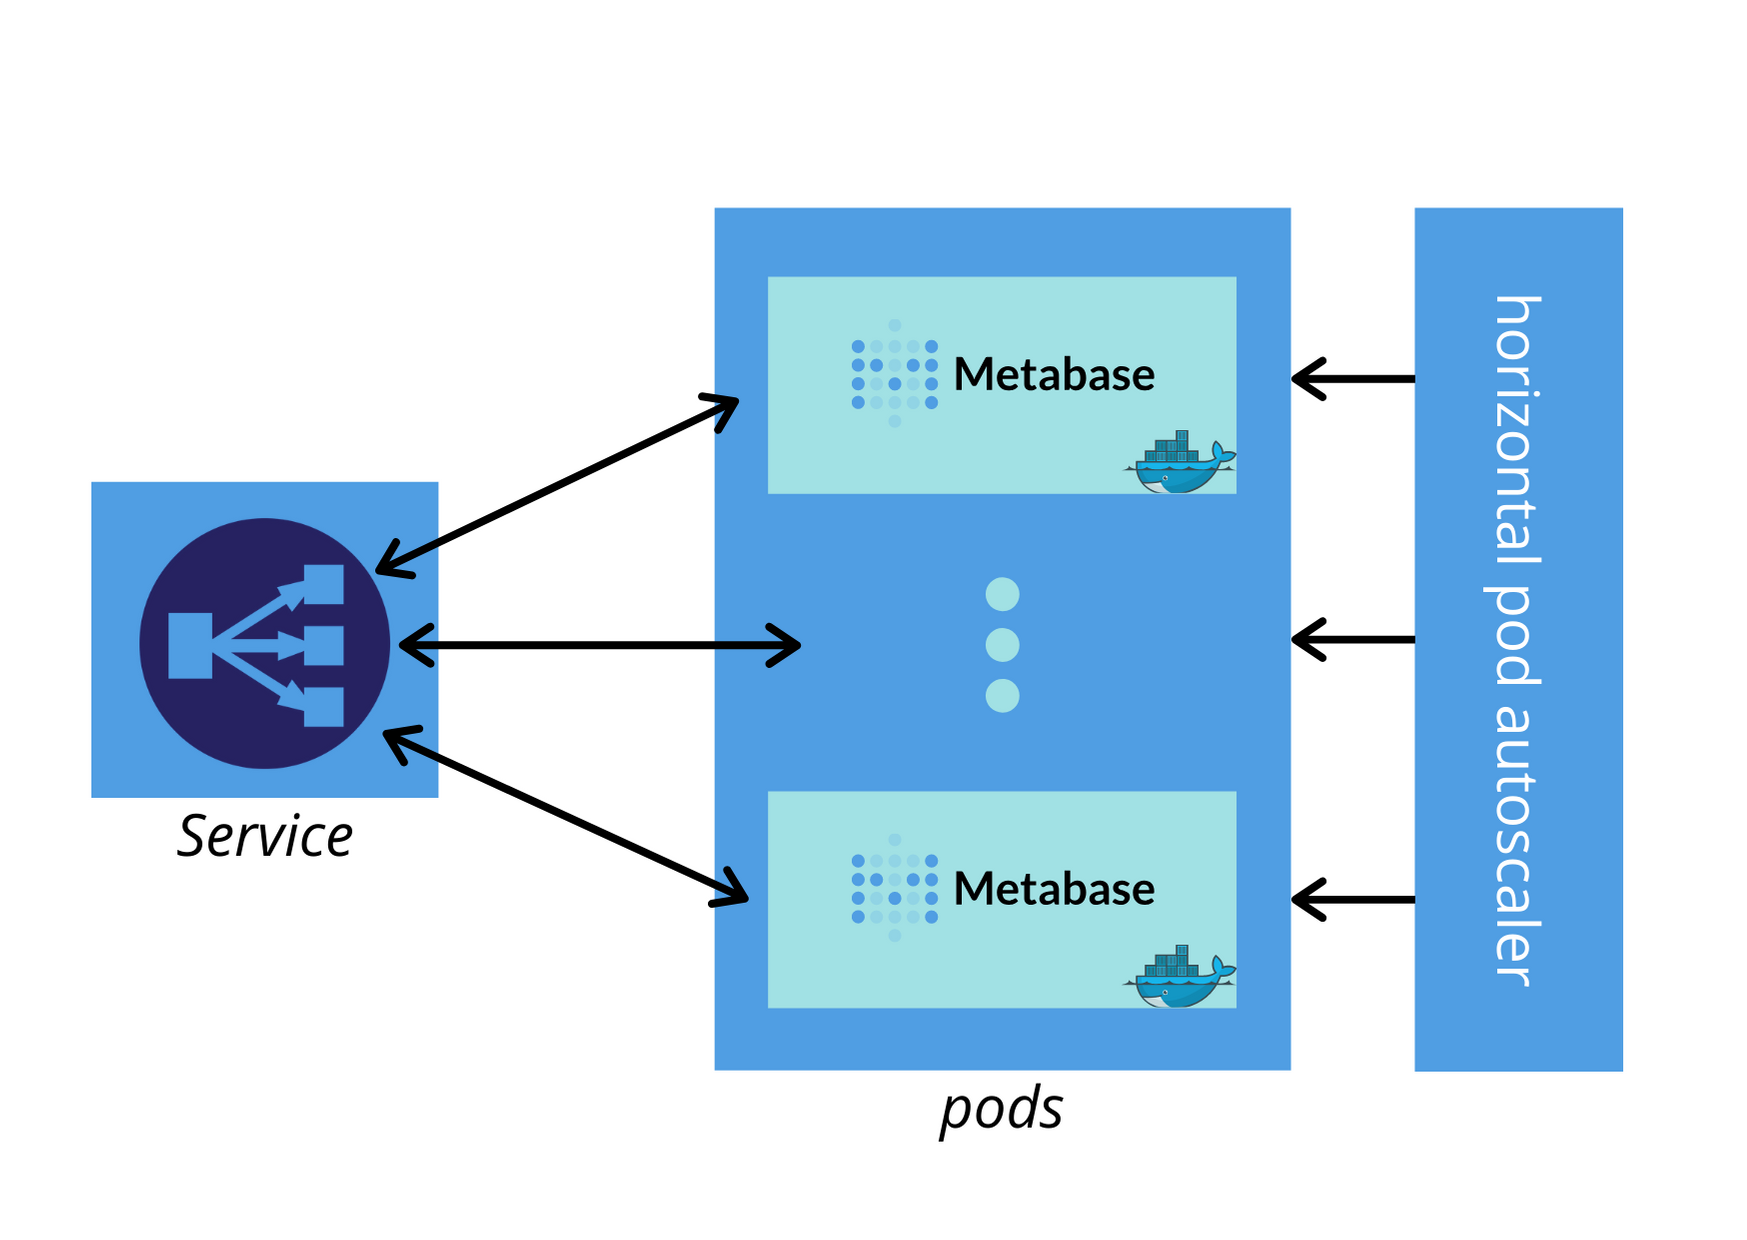
\includegraphics[width=8cm]{Imagens/Metabase-on-k8s}
    \caption{Arquitetura de implantação do Metabase em \textit{cluster} Kubernetes.}
    \label{fig.metabase-k8s}
\end{figure} 

O processo para implantação da solução proposta em um \textit{cluster} Kubernetes consiste, basicamente, na elaboração de um arquivo de configuração, em formato YAML, que descreve para o \textit{cluster} os componentes que devem ser instânciados. 

O bloco de código a seguir define um objeto \textit{configgmap} que descreve um conjunto de variávies de ambiente a serem setadas nos \textit{pods} para configuração da instância PostgreSQl que servirá de banco de dados da aplicação.

\begin{lstlisting}[language=yaml]
apiVersion: v1
kind: ConfigMap
metadata:
  name: metabase-config
  labels:
    app: metabase
data:
  MB_DB_TYPE: <DATABASE TYPE>
  MB_DB_DBNAME: <DATABASE NAME>
  MB_DB_PORT: <DATABASE PORT>
  MB_DB_USER: <DATABASE USER>
  MB_DB_PASS: <DATABASE PASSWORD>
  MB_DB_HOST: <DATABASE HOST>
\end{lstlisting} 

A seguir temos a definição do \textit{service} que será responsável pelo balanceamente de carga entre as instâncias do metabase em execução no \textit{cluster}.

\begin{lstlisting}[language=yaml]
apiVersion: v1
kind: Service
metadata:
  name: metabase-svc
spec:
  type: LoadBalancer
  selector:
    app: metabase
  ports:
    - port: 3000
      targetPort: 3000
      protocol: TCP
      name: http
\end{lstlisting} 

O arquivo com a definição do \textit{pod} do Metabase a ser executado no \textit{cluster} pode ser visto a seguir. O YAML em questão descreve algumas propriedades do \textit{pod}: a imagem base para execução do container, a porta onde o serviço será exposto, a referência do \textit{configMap} com as variáveis de ambiente, a quantidade de recursos mínimos para a aplicação e o caminho para verificação de disponibilidade do serviço. 

Por meio do rótufo \textit{spec.template.spec.resources}, são definidos os limites mínimos de recurso disponível em um \textit{node} do \textit{cluster} para que o \textit{pod} possa ser alocado, nesse caso apenas a quantidade mínima de 1 vCPU foi especificada. 

Já o rotulo \textit{spec.template.readinessProbe} defini o método pelo qual o \textit{cluster} poderá verificar a saúde da aplicação, onde nesse caso foi definido por uma requisição GET na porta 3000 no caminho '/' do container, dessa forma, o \textit{pod} só passará a receber requisições externas quando o resultado da requisição passar a ser positivo, ou seja.

\begin{lstlisting}[language=yaml]
apiVersion: apps/v1
kind: Deployment
metadata:
  name: metabase
spec:
  replicas: 1
  selector:
    matchLabels:
      deploy: metabase
  template:
    metadata:
      labels:
        deploy: metabase
        app: metabase
    spec:
      restartPolicy: Always
      containers:
        - name: metabase
          imagePullPolicy: IfNotPresent
          image: metabase/metabase:v0.35.3
          ports:
            - containerPort: 3000
          envFrom:
            - configMapRef:
                name: metabase-config
          resources:
            requests:
              cpu: 1000m
          readinessProbe:
            httpGet:
              path: /
              port: 3000
\end{lstlisting} 

Por fim, a configuração do objeto \textit{horizontal pod autoscalers} é realizada no bloco de código a seguir, descrevendo o objeto de tal forma que sempre que a média de utilização de CPU entre os \textit{pods} da aplicação sejá superior a 100\% seja adicionado um novo \textit{pod} ao conjunto, sendo permitido um conjunto mínimo de 1 \textit{pod} e máximo de 4 \textit{pods}. 

\begin{lstlisting}[language=yaml]
apiVersion: autoscaling/v1
kind: HorizontalPodAutoscaler
metadata:
  name: metabase-hpa
spec:
  scaleTargetRef:
    apiVersion: apps/v1
    kind: Deployment
    name: metabase
  minReplicas: 1
  maxReplicas: 4
  targetCPUUtilizationPercentage: 100
\end{lstlisting} 

Uma vez que todos os arquivos de configuração descritos anteriormente sejam submetidos e aceitos pelo \textit{cluster} Kubernetes, toda as operações de aumento e diminuição da quantidade de instâncias serão efetuadas automáticamente pelo \textit{control plane} do \textit{Kubernetes}.  
